
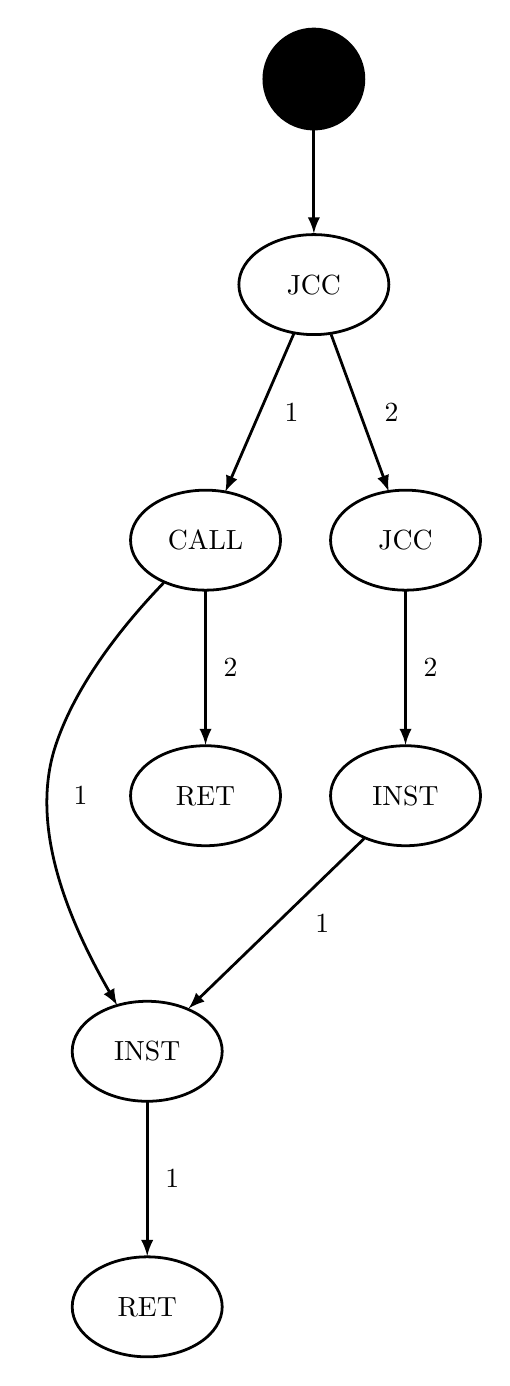
\begin{tikzpicture}[>=latex,line join=bevel,]
  \pgfsetlinewidth{1bp}
%%
\pgfsetcolor{black}
  % Edge: 2 -> 3
  \draw [->] (42.292bp,278.71bp) .. controls (29.136bp,265.07bp) and (10.954bp,243.21bp)  .. (3.3034bp,220.0bp) .. controls (-6.2298bp,191.08bp) and (7.6486bp,157.51bp)  .. (25.458bp,126.6bp);
  \definecolor{strokecol}{rgb}{0.0,0.0,0.0};
  \pgfsetstrokecolor{strokecol}
  \draw (12.303bp,202.0bp) node {1};
  % Edge: 6 -> 7
  \draw [->] (129.3bp,275.65bp) .. controls (129.3bp,262.82bp) and (129.3bp,245.11bp)  .. (129.3bp,220.3bp);
  \draw (138.3bp,248.0bp) node {2};
  % Edge: 1 -> 6
  \draw [->] (102.51bp,368.07bp) .. controls (107.33bp,354.92bp) and (114.11bp,336.43bp)  .. (123.24bp,311.55bp);
  \draw (124.3bp,340.0bp) node {2};
  % Edge: 7 -> 3
  \draw [->] (114.36bp,186.54bp) .. controls (99.311bp,171.98bp) and (75.911bp,149.33bp)  .. (51.208bp,125.42bp);
  \draw (99.303bp,156.0bp) node {1};
  % Edge: 1 -> 2
  \draw [->] (89.15bp,368.49bp) .. controls (83.378bp,355.17bp) and (75.153bp,336.19bp)  .. (64.411bp,311.4bp);
  \draw (88.303bp,340.0bp) node {1};
  % Edge: 0 -> 1
  \draw [->] (96.303bp,441.94bp) .. controls (96.303bp,433.81bp) and (96.303bp,423.88bp)  .. (96.303bp,404.44bp);
  % Edge: 2 -> 5
  \draw [->] (57.303bp,275.65bp) .. controls (57.303bp,262.82bp) and (57.303bp,245.11bp)  .. (57.303bp,220.3bp);
  \draw (66.303bp,248.0bp) node {2};
  % Edge: 3 -> 4
  \draw [->] (36.303bp,91.647bp) .. controls (36.303bp,78.823bp) and (36.303bp,61.108bp)  .. (36.303bp,36.3bp);
  \draw (45.303bp,64.0bp) node {1};
  % Node: 1
\begin{scope}
  \definecolor{strokecol}{rgb}{0.0,0.0,0.0};
  \pgfsetstrokecolor{strokecol}
  \draw (96.3bp,386.0bp) ellipse (27.0bp and 18.0bp);
  \draw (96.303bp,386.0bp) node {JCC};
\end{scope}
  % Node: 0
\begin{scope}
  \definecolor{strokecol}{rgb}{0.0,0.0,0.0};
  \pgfsetstrokecolor{strokecol}
  \definecolor{fillcol}{rgb}{0.0,0.0,0.0};
  \pgfsetfillcolor{fillcol}
  \filldraw [opacity=1] (96.3bp,460.0bp) ellipse (18.0bp and 18.0bp);
\end{scope}
  % Node: 3
\begin{scope}
  \definecolor{strokecol}{rgb}{0.0,0.0,0.0};
  \pgfsetstrokecolor{strokecol}
  \draw (36.3bp,110.0bp) ellipse (27.0bp and 18.0bp);
  \draw (36.303bp,110.0bp) node {INST};
\end{scope}
  % Node: 2
\begin{scope}
  \definecolor{strokecol}{rgb}{0.0,0.0,0.0};
  \pgfsetstrokecolor{strokecol}
  \draw (57.3bp,294.0bp) ellipse (27.0bp and 18.0bp);
  \draw (57.303bp,294.0bp) node {CALL};
\end{scope}
  % Node: 5
\begin{scope}
  \definecolor{strokecol}{rgb}{0.0,0.0,0.0};
  \pgfsetstrokecolor{strokecol}
  \draw (57.3bp,202.0bp) ellipse (27.0bp and 18.0bp);
  \draw (57.303bp,202.0bp) node {RET};
\end{scope}
  % Node: 4
\begin{scope}
  \definecolor{strokecol}{rgb}{0.0,0.0,0.0};
  \pgfsetstrokecolor{strokecol}
  \draw (36.3bp,18.0bp) ellipse (27.0bp and 18.0bp);
  \draw (36.303bp,18.0bp) node {RET};
\end{scope}
  % Node: 7
\begin{scope}
  \definecolor{strokecol}{rgb}{0.0,0.0,0.0};
  \pgfsetstrokecolor{strokecol}
  \draw (129.3bp,202.0bp) ellipse (27.0bp and 18.0bp);
  \draw (129.3bp,202.0bp) node {INST};
\end{scope}
  % Node: 6
\begin{scope}
  \definecolor{strokecol}{rgb}{0.0,0.0,0.0};
  \pgfsetstrokecolor{strokecol}
  \draw (129.3bp,294.0bp) ellipse (27.0bp and 18.0bp);
  \draw (129.3bp,294.0bp) node {JCC};
\end{scope}
%
\end{tikzpicture}

